%============================================================ 5. 실험 설계 (압축판)
%  모델명은 이 절에서 한 번만 밝히고, 이후 본문은 능력 수준(소형·중형·상위)으로 지칭한다.
%  능력 임계 주장이 특정 모델 세대나 서빙 방식에 묶이지 않게 하려는 의도다.
%  발표판은 절을 둘로만 둔다: (1) 환경과 학습 실행, (2) 조건·판정·계측.
\section{실험 설계}
\label{sec:experiment}

두 계층의 기여를 분리하기 위해 배정 축과 기동 축을 각각 이분한 $2\times2$ 조건 행렬을 두고,
시드 대응 차이로 판정한다.

\subsection{환경과 학습 실행}
\label{sec:env}
\label{sec:protocol}

%  ★ 언리얼 엔진 검증 환경의 언급과 도판(fig_ue_env)은 필수다 --- 분량을 줄일 때도 지우지 말 것.
지휘관으로는 능력 수준이 다른 소형 Qwen2.5 7B, 중형 Qwen2.5 14B, 상위 Gemini 3.5 Flash-Lite 를
온도 0, 같은 프롬프트와 구조적 출력으로 매 결정마다 호출한다. 시뮬레이터는 질점
운동학, 규칙 기반의 적, 잡음 없는 완전 관측이라 포획률은 상한이며 조건 간 상대 비교로만
판정한다. 학습과 통계 비교는 이 시뮬레이터에서 하고, 학습된 정책은 선체 거동과 충돌을 물리 엔진으로
다루는 언리얼 엔진 환경(Fig.~\ref{fig:ue_env})에서 검증한다.

\begin{figure*}[tp]
\centering
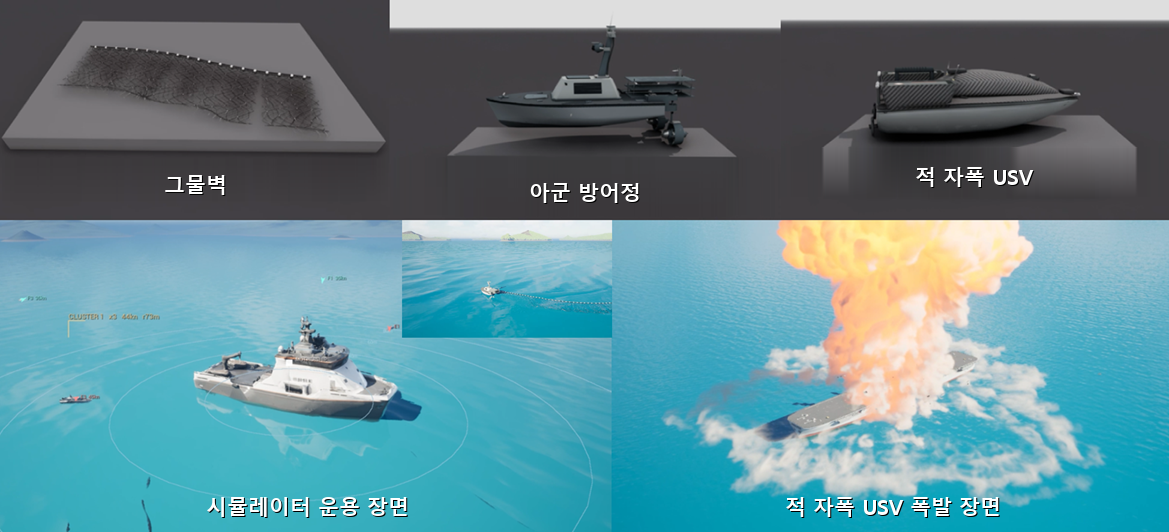
\includegraphics[width=0.92\textwidth]{fig_ue_env.png}
\caption{언리얼 엔진 기반 시뮬레이터에서의 정성 검증}
\label{fig:ue_env}
\end{figure*}


학습은 한 해안선 형상에 과적합하지 않도록 실해역 6곳(Fig.~\ref{fig:sites})을 에피소드마다
돌려가며 진행하고, 평가는 그중 통영 매물도 서측에서 한다. 총 800 업데이트 동안 주기적 greedy
평가의 최고점 가중치(600 업데이트)를 채택하였다.

\begin{figure}[!tbp]
\centering
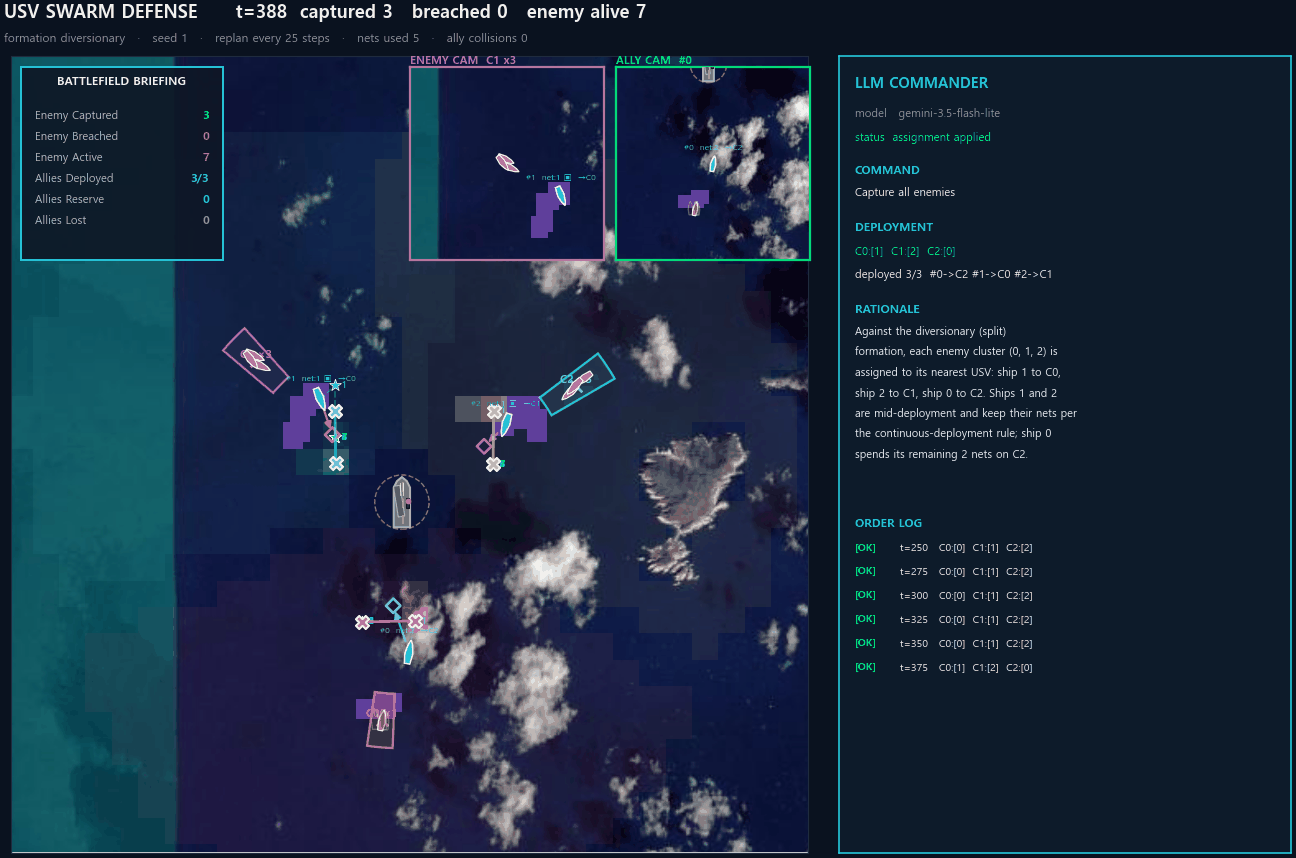
\includegraphics[width=0.75\columnwidth]{fig14.png}
\caption{학습 해역 6곳(별표 모선, 파선 원 요격 구역)}
\label{fig:sites}
\end{figure}


\subsection{조건, 판정 기준, 계측}
\label{sec:paired}
\label{sec:stats}

\begin{table}[!htb]
\centering
\caption{$2\times2$ 조건 행렬(조건 사이 차이는 두 스위치뿐)}
\label{tab:conditions}
\footnotesize
\setlength{\tabcolsep}{3pt}
\begin{tabular}{llp{0.34\linewidth}}
\toprule
조건 & 배정 $\times$ 기동 & 무엇을 측정하는가 \\
\midrule
\texttt{heur\_heur} & 휴리스틱 $\times$ 휴리스틱 & 기준선(baseline) \\
\texttt{heur\_unet} & 휴리스틱 $\times$ U-Net    & 기동 계층의 순수 기여(LLM 미사용) \\
\texttt{llm\_heur}  & LLM $\times$ 휴리스틱      & 전략 계층의 순수 기여 \\
\texttt{llm\_unet}  & LLM $\times$ U-Net         & 제안 체계(상호작용 포함) \\
\bottomrule
\end{tabular}
\end{table}

휴리스틱 배정과 기동은 \ref{sec:heuristic}절의 기준 방법이며 학습 정책과 같은 행동공간을
거치므로 네 조건은 직접 비교 가능하다(Table~\ref{tab:conditions}). 전략 계층에 세 모델을 두고
모든 조건이 같은 시드 집합과 세 포메이션을 공유하도록 하여 720 에피소드를 수집하였다.

조건과 기준선의 시드 $k$ 지표값을 $x_k$, $y_k$, 시드 수를 $n_{\mathrm{s}}$, 대응 차이 $d_k$ 의
표준편차를 $s_d$ 라 하면 차이의 평균과 효과크기는
\begin{equation}
d_k = x_k - y_k, \qquad
\bar{d} = \frac{1}{n_{\mathrm{s}}}\sum_{k} d_k, \qquad
\dz = \frac{\bar{d}}{s_d}
\label{eq:paired}
\end{equation}
이며, 95\,\% 신뢰구간은 BCa 부트스트랩~\citep{efron1993bootstrap}($B = 9999$)으로 구하고
지표 9개의 다중비교에는 Bonferroni 보정 구간(99.4\,\%)을 병기한다. 상호작용은 배정 축(H 휴리스틱,
L 언어모델)과 기동 축(H 휴리스틱, U U-Net)의 조건별 지표값 $x_k^{am}$ 에서
\begin{equation}
\mathrm{Int}_k = \big(x_k^{\mathrm{LU}} - x_k^{\mathrm{LH}}\big)
               - \big(x_k^{\mathrm{HU}} - x_k^{\mathrm{HH}}\big)
\label{eq:interaction}
\end{equation}
로 같은 절차를 거쳐 판정한다($>0$ 상승, $\approx 0$ 가산, $<0$ 상쇄).

지휘관 계층은 포획률만으로 기여가 가려지므로 응답 지연, 폴백률(언어모델 실패로 휴리스틱이 대체한
비율), 커버리지(활성 무리 중 배정된 비율), churn(재계획 간 담당을 바꾼 방어정 비율), 교차 배정을
따로 계측한다.
